\section{Proposed Method}

%Introduction

In the proposed method of remastered song identification, various algorithms are used to
extract the audio features, create audio descriptors and match against stored descriptors.
Hence we have divided our remastered song identification process in to five steps.

\begin{enumerate}
    \item Preprocessing
    \item Feature Extracting
    \item Descriptor Storing (Registering)
    \item Matching
    \item Postprocessing
  \end{enumerate}

Processes of the above steps will be discussed in the following subsections.

\begin{figure}[h]
    \centering
    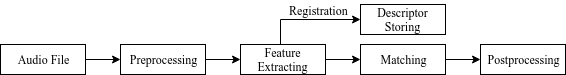
\includegraphics[scale=0.4]{research_paper/graphics/pipeline.png}
    \caption{Remastered Song Identification Process}
    \label{fig:pipeline}
\end{figure}


\subsection{Preprocessing}
%STFT

In default audio data is represented in the time domain. Since even a small change in an audio changes the time domain representation drastically,
using the time domain representation of the audio to extract features is not recommended. Hence time domain audio signal is converted to
frequency domain signal by using \gls{stft} method. \gls{stft} is a sequence of Fourier transforms of a windowed signal\cite{Kehtarnavaz2008}.
2048 bits long window with 50\% overlapping was used as \gls{stft} key parameters as depicted in Figure \ref{fig:parameters}.

\begin{figure}[h]
  \centering
  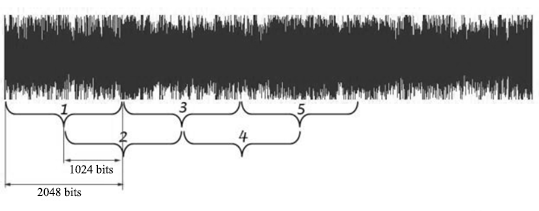
\includegraphics[scale=0.6]{research_paper/graphics/parameters.png}
  \caption{Key parameters on \gls{stft}. 2048 bits long window with 1024 bits long overlapping area.}
  \label{fig:parameters}
\end{figure}

\gls{stft} is often visualized using its spectrogram\cite{Kehtarnavaz2008}, which is an intensity plot of \gls{stft} magnitude over time. 
The generated spectrogram is converted to a color image as shown in Figure \ref{fig:spectrogram}. Axis labels and ticks are removed to stop
identification of them as key points in feature extracting step. 

\begin{figure}[h]
  \centering
  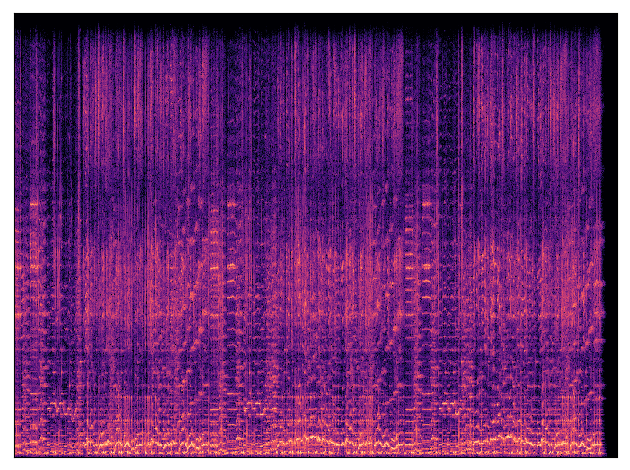
\includegraphics[scale=0.5]{research_paper/graphics/spectrogram.png}
  \caption{Generated colour image of spectrogram after preprocessing.}
  \label{fig:spectrogram}
\end{figure}

\subsection{Feature Extracting}
%SIFT

\gls{stft} spectrogram itself can be considered as an audio descriptor\cite{Ke2005}. This method uses \gls{sift}\cite{Lowe2004} to extract 
the features which are robust to music remastering. In the Figure \ref{fig:compare_spectrogram}, it can be observed that when tempo is
altered the spectrogram will either expand or compress with the time axis and when pitch is altered the spectrogram will either shift upwards or 
downwards with the frequency axis. 

\begin{figure}[h]
  \centering
  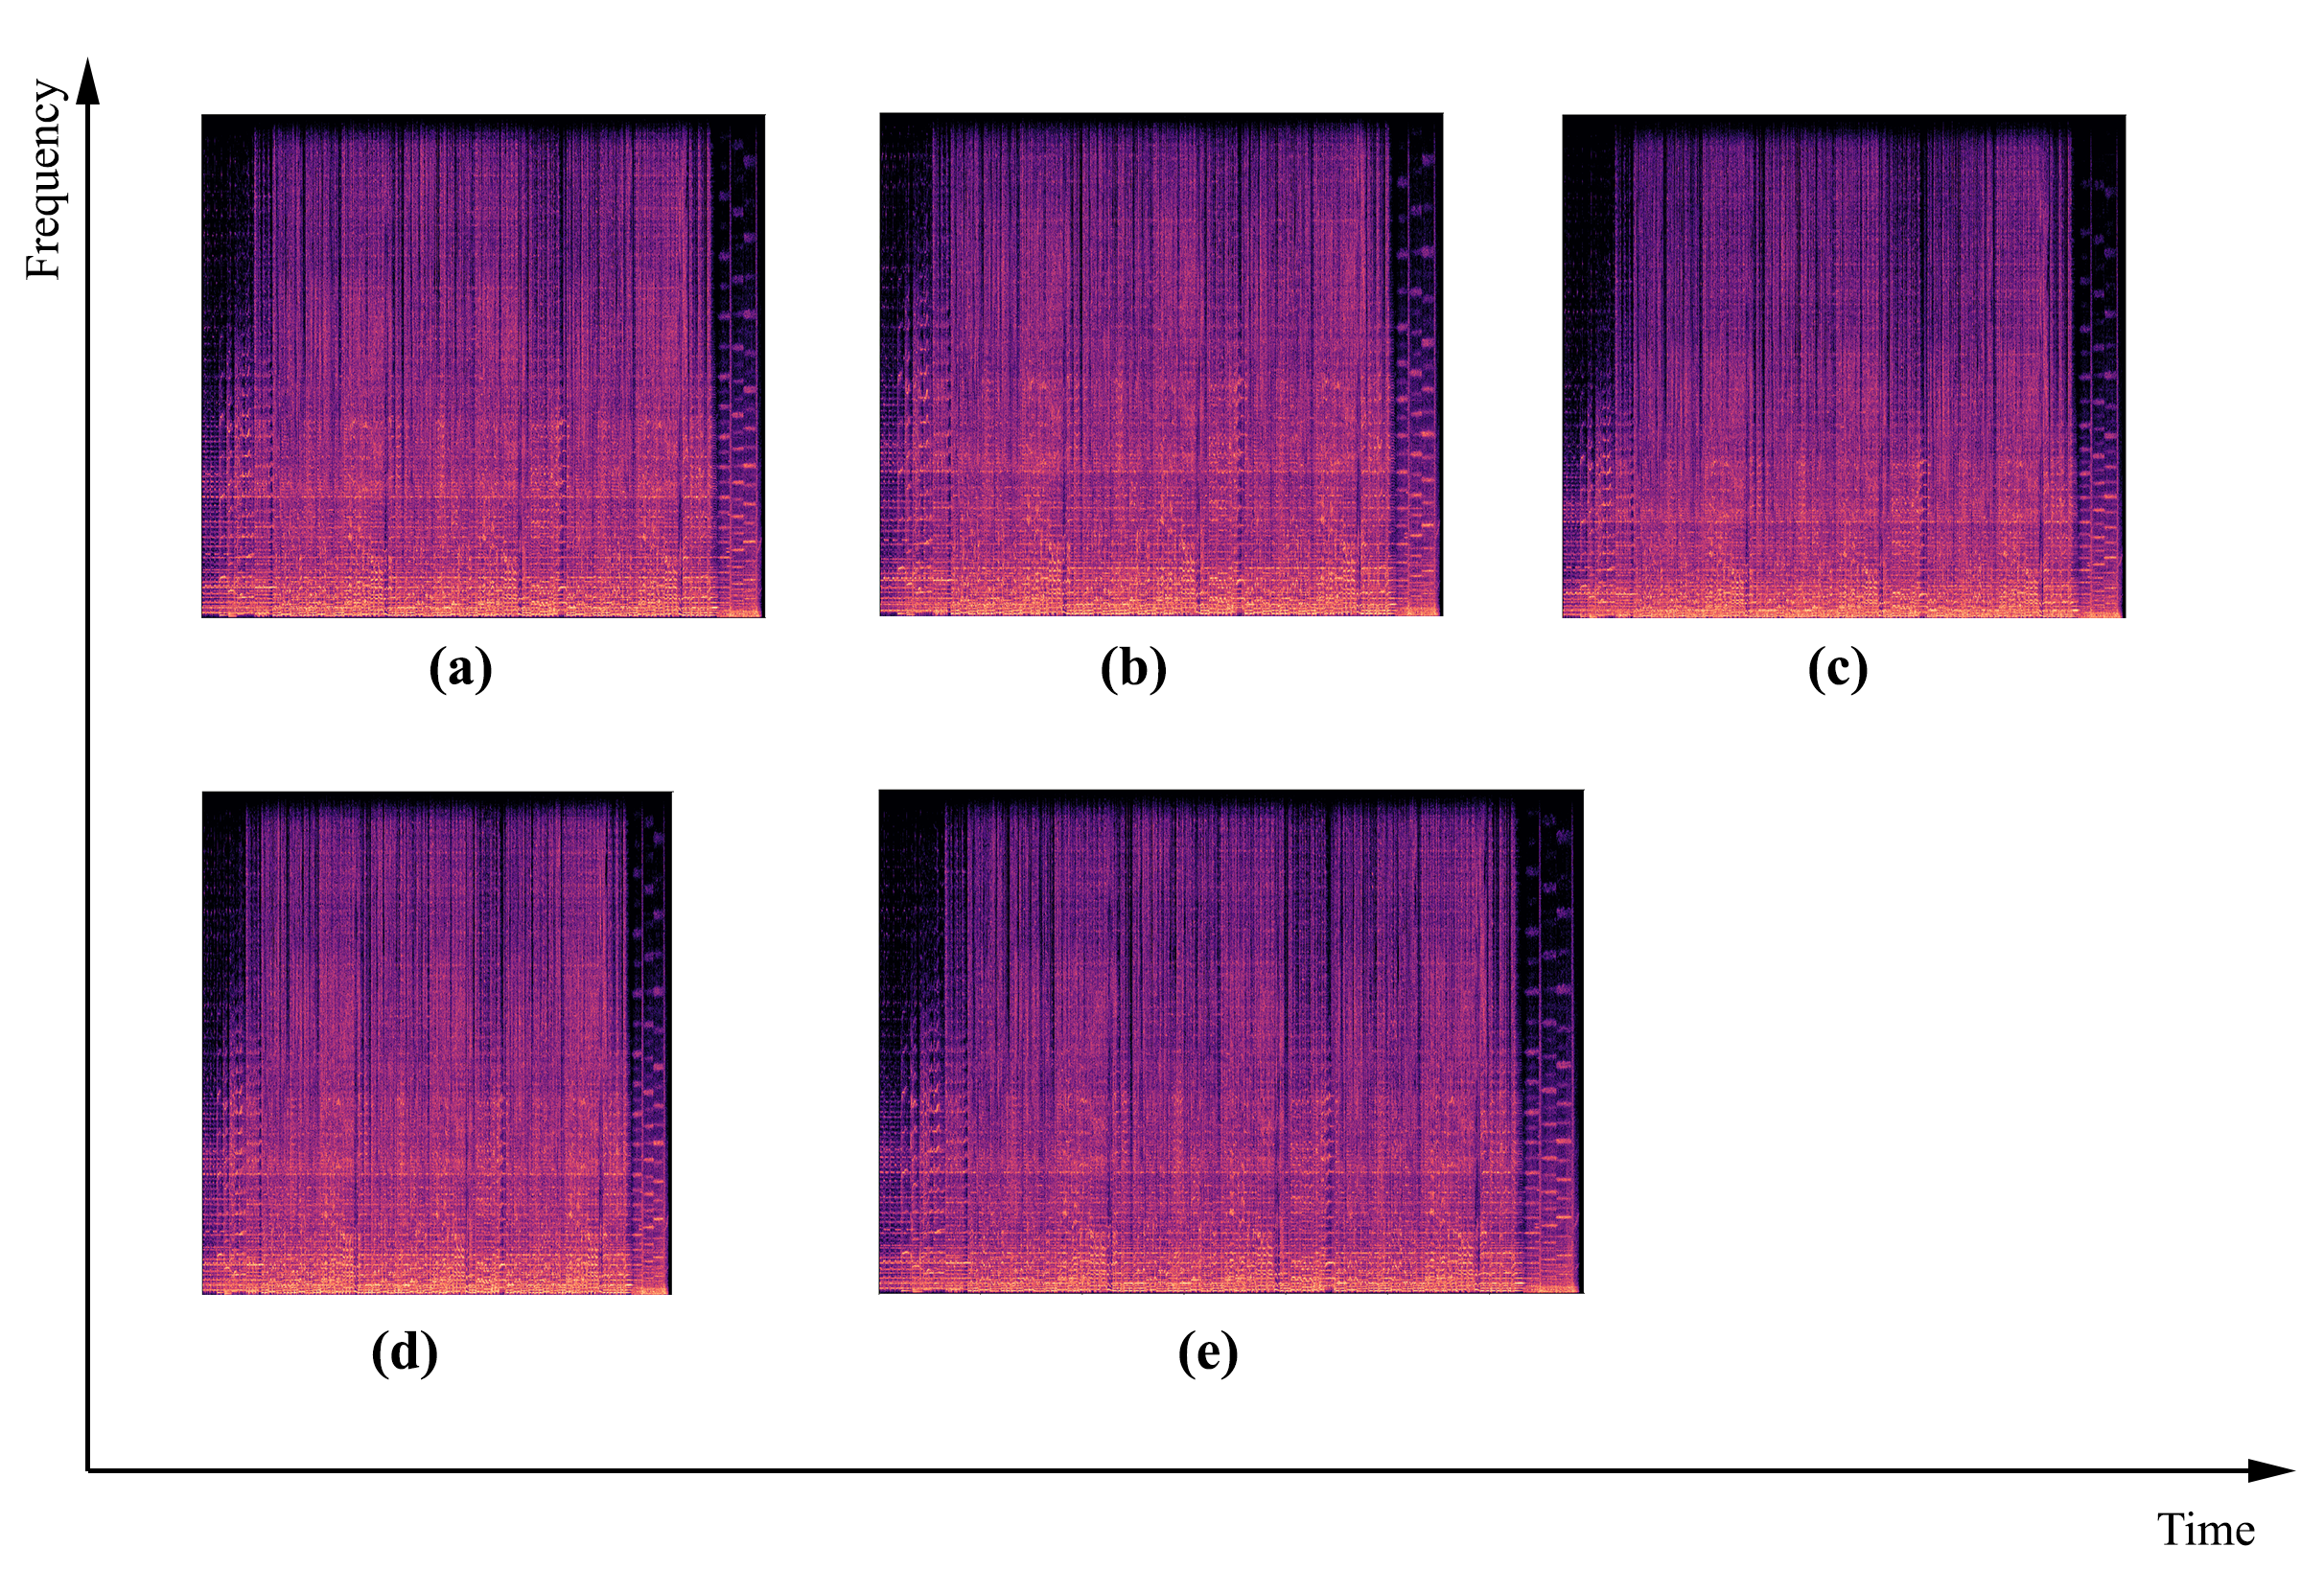
\includegraphics[scale=0.4]{research_paper/graphics/spec_transform.png}
  \caption{Spectrogram transformations on audio enhancements. \textbf{(a)} is the spectrogram image of a original song. \textbf{(b)} 20\% 
  pitch increase, \textbf{(c)} 20\% pitch decrease, \textbf{(d)} 20\% tempo increase and \textbf{(e)} 20\% tempo decrease spectrogram images.}
  \label{fig:compare_spectrogram}
\end{figure}

\gls{sift} is used in computer vision to identify scale invariant features of an image. \gls{sift} features are invariant to image rotation,
scale alterations and illumination\cite{Lowe2004}. The \gls{sift} feature extractor used in this method consists of four main steps.
\begin{enumerate}
  \item Scale space extrema detection: Gaussian filters of different scales are applied to the image and potential key points are selected
  as local minima or maxima of the \gls{dog} for multiple scales.
  \item Keypoint localization: Keypoints that have low contrast or those that are poorly located along edges
  are filtered out.
  \item Orientation assignment: One or more orientations are assigned to each keypoint based on local image gradient. 
  \item Keypoint descriptor generation: Orientation histograms are created for 4 x 4 pixel neighborhoods for each keypoint.
  Each histogram consists 8 bins, hence (4 x 4 x 8) 128 dimensional descriptor is generated.
\end{enumerate}

A Set of extracted 128 dimensional descriptors works together in describing the input audio file. Extracted 
\gls{sift} features are invariant to image stretch and translation which makes them better features to be used
in audio identification algorithm which is robust to tempo alterations and pitch shifting. 

\subsection{Descriptor Storing (Registering)}
\gls{sift} descriptors of original songs must be stored to use them in the matching step of the remastered
song identification process. Generally 3-5 minute music clip will have around 2000 key points in its \gls{stft}
spectrogram. Hence a \(2000\times 128\) matrix will be generated for each original song that will be registered.

The descriptor matrix of each original song is converted to a binary string and that binary string is stored 
in the database as \gls{blob}s. Converting to binary string and storing the matrix as a \gls{blob} will ensure
fast recreation of the matrix while retrieving\cite{Sears2006}.   

\subsection{Matching}
%Final Result
Music identification is facilitated by matching a feature matrix of a query audio clip with a feature matrix of a original song. Final goal
of the matching is to identify the count of keypoints that are matched with the original song. Identification of matching keypoints achieved
by taking 2 nearest keypoints to a query keypoint and checking whether the distance to the closest keypoint is lesser than 
the \(0.75 \times \text{distance to the 2nd closest keypoint}\).

\subsection{Postprocessing}
%Variable Tuning
the most similar song and matched keypoint count for a given query audio clip is identified in the matching step. But
it doesn't exactly mean that query audio clip contains that song. Because the number of keypoints that were matched
represents how much the query song matched to the most similar song. Hence there should be a threshold keypoint count
to determine whether a query audio clip contains a song in our database or not. But using just a threshold value 
won't work here since different query audio clips generate different number of key points to match against the
database. Hence ratio based threshold is recommended as a measure to determine whether the matched song is actually a
correct match. Keypoint ratio can be obtained by the below equation. 

\begin{align*}
\text{Keypoint ratio} &= \frac{\text{Matched keypoint count}}{\text{Keypoints generated for query audio clip}}\\
\end{align*}

Based on this keypoint ratio, a threshold is used to determine the validity of the match found. In order to find this
threshold value we have used 844 different audio clips with variable durations to match against 2300 original songs.
Those 844 audio clips had 519 audio clips which had songs and 325 audio clips which didn't have songs from those 
2300 original songs. And we calculated accuracy for 18 testcases which will be discussed in section 
\ref{section:experiments}, and took average of those 18 accuracies for variable threshold values. Then results were
illustrated as shown in the Figure \ref{fig:threshold}. 

\begin{figure}[h]
  \centering
  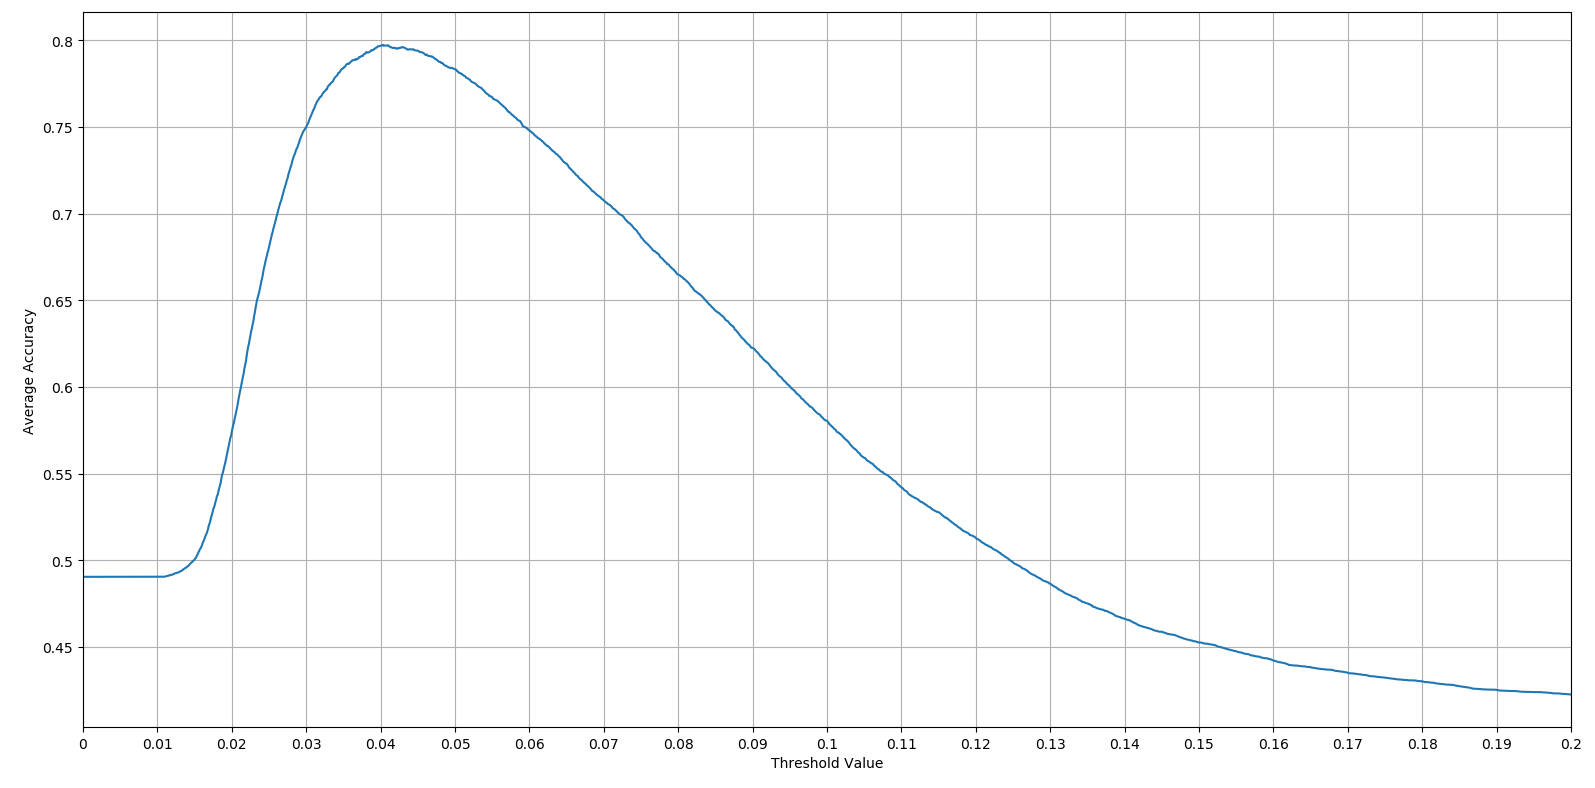
\includegraphics[scale=0.21]{images/threshold_adjusting.png}
  \caption{Average Accuracy Values for Different Threshold Values}
  \label{fig:threshold}
\end{figure}

Global peak can be observed in the illustration which makes that value a clear threshold point. 0.0298 is the threshold
value that was found. Hence if keypoint ratio of a query audio is larger than 0.0298 then it's identified as a valid match
to the song that was identified in the matching step, otherwise it's identified as a invalid match. This threshold point
makes this method to clearly identify whether a query audio has a song which is in a database or not.  